% MIT License

% Copyright (c) 2022 Chiyuru

% Permission is hereby granted, free of charge, to any person obtaining a copy of this software and associated documentation files (the "Software"), 
% to deal in the Software without restriction, including without limitation the rights
% to use, copy, modify, merge, publish, distribute, sublicense, and/or sell
% copies of the Software, and to permit persons to whom the Software is
% furnished to do so, subject to the following conditions:

% The above copyright notice and this permission notice shall be included in all copies or substantial portions of the Software.

% THE SOFTWARE IS PROVIDED "AS IS", WITHOUT WARRANTY OF ANY KIND, EXPRESS OR IMPLIED, INCLUDING BUT NOT LIMITED TO THE WARRANTIES OF MERCHANTABILITY,
% FITNESS FOR A PARTICULAR PURPOSE AND NONINFRINGEMENT. IN NO EVENT SHALL THE AUTHORS OR COPYRIGHT HOLDERS BE LIABLE FOR ANY CLAIM, DAMAGES OR OTHER
% LIABILITY, WHETHER IN AN ACTION OF CONTRACT, TORT OR OTHERWISE, ARISING FROM,
% OUT OF OR IN CONNECTION WITH THE SOFTWARE OR THE USE OR OTHER DEALINGS IN THE SOFTWARE.

\documentclass[UTF8]{ctexart}
\setcounter{tocdepth}{2}

\usepackage{amsmath}
\usepackage{amssymb}
\usepackage{colortbl}
\usepackage{array}
\usepackage{cases}
\usepackage{cite}
\usepackage{diagbox}
\usepackage{graphicx}
\usepackage{booktabs}
\usepackage{float}
\usepackage{subcaption}
\usepackage{tabularx}
\usepackage{threeparttable}
\usepackage{listings}
\usepackage{multirow}
\usepackage{enumitem}
\usepackage{xcolor}
\usepackage{url}
\usepackage[margin=1in]{geometry}
\geometry{a4paper}
\usepackage{fancyhdr}
\pagestyle{fancy}
\fancyhf{}
\setlength{\headheight}{13pt}

\usepackage{matlab}

\lstset{
    basicstyle=\ttfamily\footnotesize,
    backgroundcolor=\color{gray!10},
    frame=single,
    rulecolor=\color{black},
    breaklines=true,
    postbreak=\mbox{\textcolor{red}{$\hookrightarrow$}\space},
}

\newcommand{\code}[1]{\texttt{\detokenize{#1}}}

\title{Advanced Topics for Robotics Homework 2}
\author{Yixuan Li}
\date{April 25, 2026}
\pagenumbering{arabic}
\renewcommand{\figurename}{Figure}
\renewcommand{\tablename}{Table}
\urlstyle{tt}
\graphicspath{{report/images/}{images/}{./}}

\setlength{\parindent}{0pt}
\setlength{\parskip}{0.6em}

\begin{document}

\fancyhead[L]{HW2}
\fancyhead[R]{Yixuan Li \, 2023010651}
\fancyfoot[C]{\thepage}

\maketitle
\renewcommand{\contentsname}{Contents}
\setcounter{tocdepth}{3}
{
\linespread{1}\selectfont
\setlength{\parskip}{2pt}
\tableofcontents
}

\newpage
\section{Dataset Preparation}

This homework uses the RobotEra M7 pick-and-place demonstrations as an imitation-learning dataset. The raw demonstrations were converted into a zarr replay buffer so that the Diffusion Policy dataloader can index image observations, low-dimensional robot state, and action chunks with the same interface used by the original benchmark code.

The final dataset used in the main experiments is \code{data/m7_3cam.zarr}. It contains 491 episodes. Each training sample contains three camera streams, a proprioceptive state vector, and an action sequence. The image observations are resized to \(96 \times 96\) and exposed as three RGB keys: \code{cam_high}, \code{cam_left}, and \code{cam_right}. The state vector has dimension 57 and the action vector has dimension 38. The policy therefore observes both visual object context and robot configuration, while predicting a short future action chunk.

The custom dataloader is \code{M7Star1Dataset}. It reads the zarr replay buffer, maps the three camera keys to the image arrays stored in the buffer, validates the expected state and action shapes, and builds a \code{SequenceSampler} with the configured horizon and padding. For controlled data splits, the dataloader supports both explicit episode ranges and random downsampling. The episode range is inclusive: \code{episode_start=0, episode_end=365} uses episodes 0--365. This is used to separate the clean apple-box subset, the larger mixed subset, and the full dataset.

\begin{table}[H]
    \centering
    \caption{Dataset variants used in the report}
    \label{tab:dataset-variants}
    \small
    \begin{tabularx}{\linewidth}{lXcc}
        \toprule
        Variant & Selection rule & Episodes used for training & Purpose \\
        \midrule
        DP-base & \code{episode_start=0, episode_end=365} & 366 & Clean apple-box subset \\
        DP-mix & \code{episode_start=0, episode_end=449} & 450 & Larger apple-box/mixed subset \\
        DP-full & \code{episode_start=0, episode_end=490} & 491 & Full dataset baseline \\
        DP-10 & \code{max_train_episodes=49} & 49 & 10\% data-efficiency study \\
        DP-50 & \code{max_train_episodes=246} & 246 & 50\% data-efficiency study \\
        \bottomrule
    \end{tabularx}
\end{table}

The validation split deserves one implementation note. The training mask is formed from the selected episode mask, but the validation dataset is built from the complement of the final training mask. As a result, DP-base validates not only on the small held-out portion of episodes 0--365, but also on episodes 366--490, which are outside its training distribution. This was an implementation mistake, making its validation loss much harder to interpret than its training loss. In contrast, DP-full validates mostly on the held-out split of the same overall distribution.

\section{Training Diffusion Policy}

The main policy is based on the image-conditioned Diffusion Policy architecture. I used a transformer hybrid image policy instead of a pure low-dimensional policy because the task requires visual localization of the object and target region. The configuration uses a prediction horizon of 10, two observation steps, and eight action steps. Each observation contains the three RGB camera images and the 57-dimensional robot state. The diffusion scheduler is DDPM with 100 training timesteps in the baseline, and the policy performs 100 denoising steps at inference time unless otherwise specified.

The base transformer has 8 layers, 4 attention heads, and an embedding size of 256. The image encoder uses a \(76 \times 76\) crop and group normalization. The optimizer uses learning rate \(10^{-4}\), batch size 64, seed 42, EMA enabled, and checkpointing every 50 epochs. All experiments were launched with Hydra overrides rather than editing the YAML files directly.

\begin{table}[H]
    \centering
    \caption{Training experiments}
    \label{tab:training-experiments}
    \scriptsize
    \resizebox{\linewidth}{!}{
    \begin{tabular}{llll}
        \toprule
        ID & Config & Key override & Question answered \\
        \midrule
        DP-base & \code{image_m7_star1.yaml} & episodes 0--365 & Clean-subset baseline \\
        DP-mix & \code{image_m7_star1.yaml} & episodes 0--449 & Larger mixed-subset baseline \\
        DP-full & \code{image_m7_star1.yaml} & episodes 0--490 & Full-data baseline \\
        DP-10 & \code{image_m7_star1.yaml} & \code{max_train_episodes=49} & 10\% data efficiency \\
        DP-50 & \code{image_m7_star1.yaml} & \code{max_train_episodes=246} & 50\% data efficiency \\
        DP-trn50 & \code{image_m7_star1.yaml} & \code{num_train_timesteps=50} & Diffusion training steps \\
        DP-inf50 & \code{image_m7_star1.yaml} & \code{num_inference_steps=50} & Inference sampling budget \\
        DP-depth4 & \code{image_m7_star1.yaml} & \code{policy.n_layer=4} & Network depth \\
        BC-100 & \code{bc_m7_star1.yaml} & full dataset & Behavior Cloning baseline \\
        \bottomrule
    \end{tabular}}
\end{table}

The three dataset baselines separate different sources of task ambiguity. DP-base uses the clean apple-to-box demonstrations, where one hand grasps the apple and places it into the box. DP-mix includes more apple-box demonstrations, including cases where one hand interacts with the apple while the other hand interacts with the box. DP-full further includes demonstrations with another graspable object, such as mango. Since this Diffusion Policy setup does not receive a language token, the full dataset can make the rollout target ambiguous when multiple objects are visible. For this reason, DP-base is the most directly matched baseline for the final apple-to-box evaluation scene.

\begin{figure}[H]
    \centering
    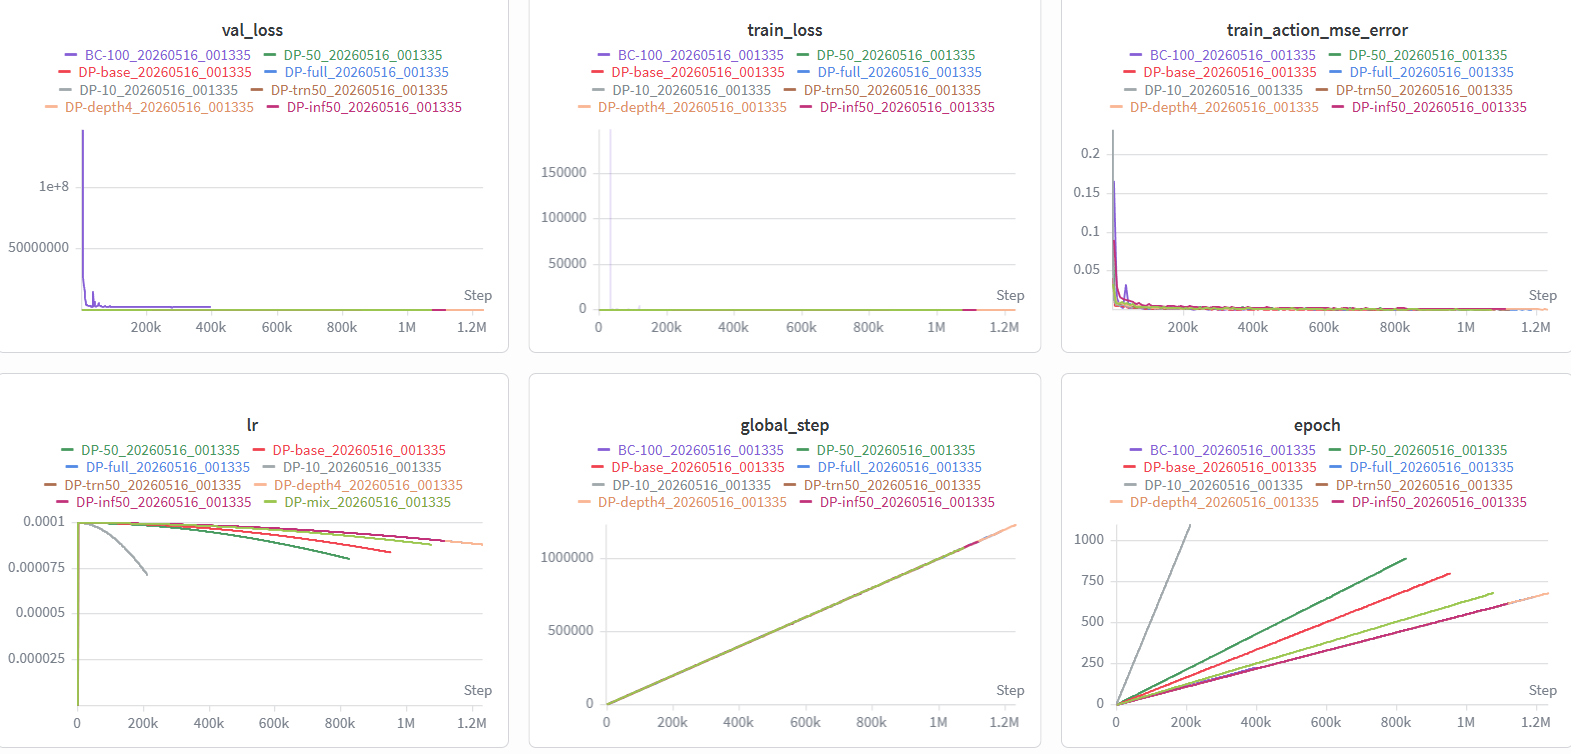
\includegraphics[width=1\linewidth]{full_train_curve.png}
    \caption{Training curves for all DP and BC runs. The large BC loss scale compresses the DP curves in the loss plots.}
    \label{fig:all-train-curves}
\end{figure}

\begin{figure}[H]
    \centering
    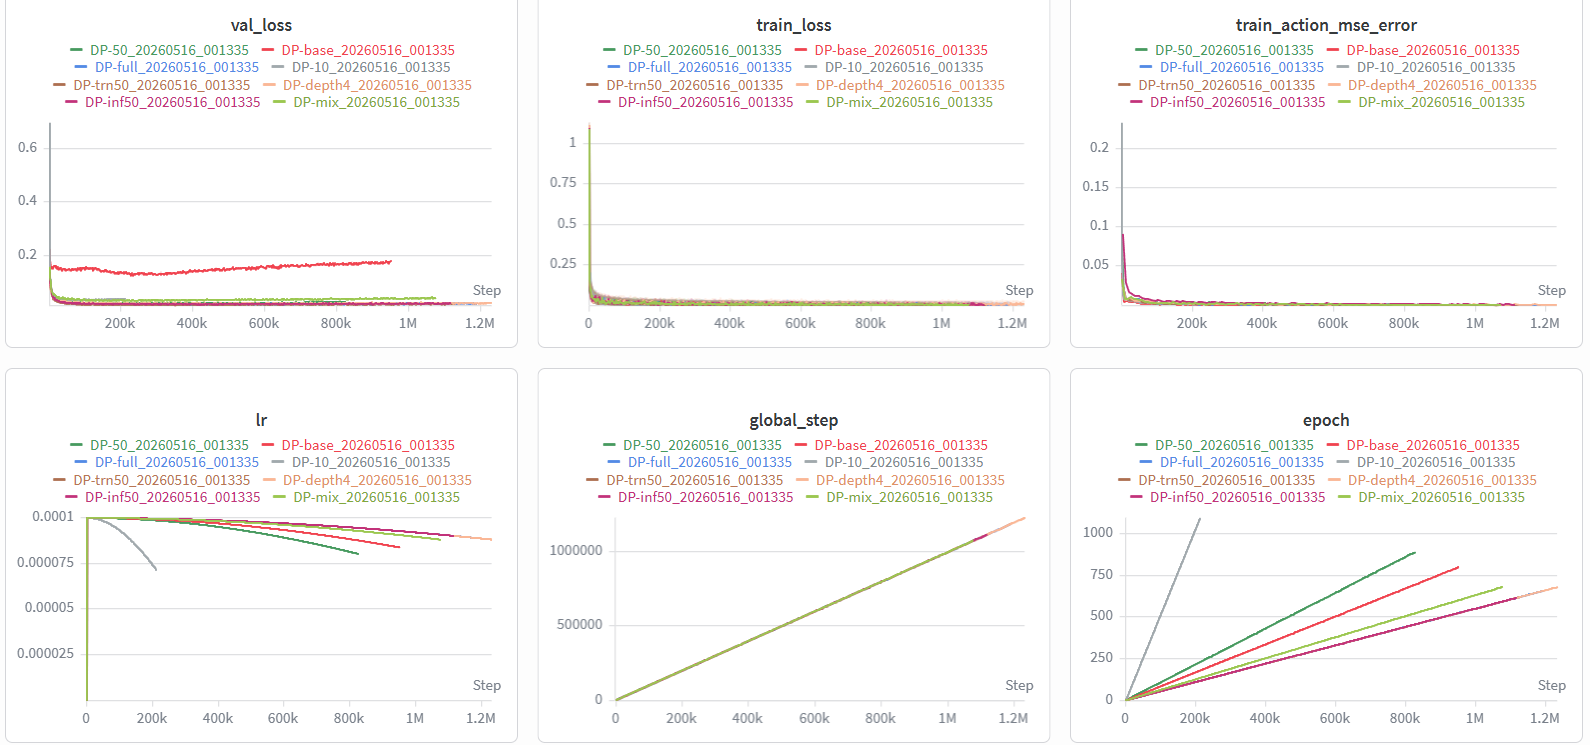
\includegraphics[width=1\linewidth]{full_dp_train_curve.png}
    \caption{Training curves for the DP runs only, shown without BC so that DP validation loss, training loss, action MSE, learning rate, global step, and epoch trends are readable.}
    \label{fig:dp-train-curves}
\end{figure}

Figure~\ref{fig:all-train-curves} shows why BC is analyzed separately: its loss values and spikes are much larger than the DP losses, so it dominates the shared y-axis. Figure~\ref{fig:dp-train-curves} shows that the DP runs all reduce training loss quickly and then improve more slowly. With the current training budget, the final DP training losses are generally in the \(10^{-3}\) to \(10^{-2}\) range. Smaller data subsets advance through epochs faster because each epoch contains fewer batches, while their validation losses are harder to interpret because of the validation-mask behavior discussed after Table~\ref{tab:dataset-variants}.

\begin{table}[H]
    \centering
    \caption{Training metrics at the selected latest checkpoints}
    \label{tab:train-metrics}
    \scriptsize
    \resizebox{\linewidth}{!}{
    \begin{tabular}{lrrrrl}
        \toprule
        Run & Selected epoch & Train loss & Validation loss & Action MSE & Observation \\
        \midrule
        DP-base & 850 & 0.00564 & 0.17835 & 0.00022 & Lowest action MSE; validation hardest because it includes unseen episodes \\
        DP-mix & 750 & 0.00561 & 0.04028 & 0.00054 & Stable apple-box subset fit with moderate validation loss \\
        DP-full & 700 & 0.00573 & 0.02071 & 0.00047 & Best full-distribution validation among the main baselines \\
        DP-10 & 1050 & 0.01011 & 0.03610 & 0.00157 & Less data coverage and higher action error \\
        DP-50 & 1000 & 0.00584 & 0.02678 & 0.00070 & Close training fit, but less coverage than full data \\
        DP-trn50 & 700 & 0.00425 & 0.02316 & 0.00048 & Lower training loss with shorter diffusion training chain \\
        DP-inf50 & 650 & 0.00591 & 0.02285 & 0.00089 & Similar validation loss with reduced inference sampling budget \\
        DP-depth4 & 750 & 0.00866 & 0.02025 & 0.00092 & Smaller model with weaker training fit \\
        BC-100 & 250 & -250.753 & \(2.264 \times 10^{6}\) & 0.00071 & Low action MSE but unstable long-horizon rollout \\
        \bottomrule
    \end{tabular}}
\end{table}

DP-base has much higher validation loss than DP-full even though its training loss is comparable. This is caused by the validation-mask behavior described above: the base model is evaluated on episodes outside the clean subset, so its validation loss partly measures out-of-distribution generalization. DP-10 also converges to a higher training loss, which is expected because 49 episodes do not cover the same diversity of object poses, contacts, and approach trajectories.

\section{Evaluation}

The evaluation setup uses a policy server and the XBot simulation benchmark. The policy server loads a trained checkpoint, receives the three camera observations and robot state, and returns action chunks. The simulator then executes the action sequence in the pick-and-place scene. The same evaluation scene should be used for all variants so that the comparison reflects policy behavior rather than differences in object placement or rendering.

\begin{table}[H]
    \centering
    \caption{Expected rollout behavior in the apple-to-box evaluation setting}
    \label{tab:eval-behavior}
    \scriptsize
    \resizebox{\linewidth}{!}{
    \begin{tabular}{ll}
        \toprule
        Run & Expected rollout behavior \\
        \midrule
        DP-base & Best matched to the apple-to-box scene; should choose the apple most consistently and avoid object-selection ambiguity \\
        DP-mix & Should retain strong apple-box behavior but may be slightly less consistent because the demonstrations include more interaction patterns \\
        DP-full & Should benefit from more data diversity but may confuse the target object when multiple graspable objects are visible \\
        DP-trn50 & Should behave similarly to DP-full, with a shorter training diffusion chain that may be easier to optimize but less expressive \\
        DP-inf50 & Should behave similarly to DP-full during approach motion, with faster sampling but slightly less final-action refinement \\
        DP-depth4 & Should be weaker in camera-state fusion and late contact correction because of reduced transformer capacity \\
        DP-50 & Should cover the main approach behavior but be less robust to rare object poses and contact timings than DP-full \\
        DP-10 & Should have the weakest data coverage and therefore the least reliable contact and placement behavior \\
        BC-100 & Should fit local actions but be weakest at long-horizon recovery after small deviations from the demonstration distribution \\
        \bottomrule
    \end{tabular}}
\end{table}

All rollout success rates were 0 in the final evaluation. The most meaningful behaviors still came from DP-base and DP-mix: the hand hesitated near the start pose and showed a small but visible tendency to move toward the target object. The remaining variants were less stable and often produced hand motions that quickly left the useful workspace. Compared with a simpler two-finger gripper setup, the dexterous hand has many more degrees of freedom, so the same loss scale is not enough to guarantee stable rollout. The results therefore mainly indicate under-trained long-horizon control rather than a complete absence of task signal.

\begin{figure}[H]
    \centering
    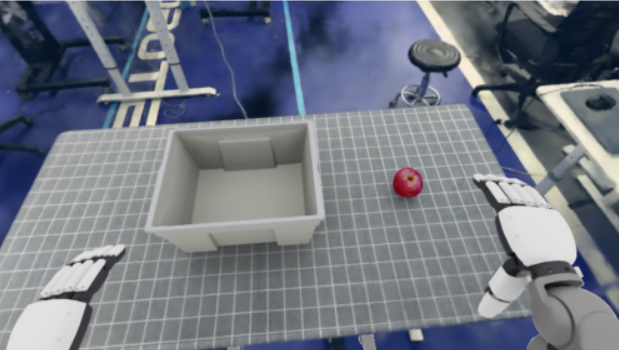
\includegraphics[width=0.5\linewidth]{3d_eval.png}
    \caption{Apple-to-box evaluation scene with the target box and apple visible from the high camera.}
    \label{fig:eval-scene}
\end{figure}

I also trained a DP-full variant using only \code{cam_high}, which reduced the training load and allowed faster epoch iteration. Even after 1450 epochs, this single-camera model still showed hesitant motion with only slight progress toward the object. This suggests that the failure was not caused only by the three-camera input cost; the dexterous manipulation policy likely needed either substantially more optimization or a more constrained action representation.

\section{Analysis}

\subsection{Hyperparameter Analysis}

\paragraph{Diffusion training steps.} DP-trn50 changes the DDPM training timesteps from 100 to 50. Its intermediate validation loss is slightly lower than DP-full, which suggests that the shorter denoising chain is easier to optimize on this dataset. This does not automatically mean that it will be better in rollout. A smaller number of training timesteps may reduce the expressivity of the denoising process, especially when the policy must model several valid approach directions. Based on the training curves, DP-trn50 is stable and should be competitive with DP-full.

\paragraph{Inference denoising steps.} DP-inf50 keeps the training objective unchanged but reduces the number of inference denoising steps from 100 to 50. Its validation loss remains close to DP-full, as expected, because validation loss is mostly tied to the trained denoising objective rather than the sampling budget. The practical trade-off is inference latency versus final action refinement. In rollout, DP-inf50 should be nearly as stable as DP-full during approach motion, but may be slightly worse during the final contact and placement correction, where additional denoising steps can smooth small residual errors.

\paragraph{Network depth.} DP-depth4 reduces the transformer from 8 layers to 4. It still learns the task, but its validation loss is higher than DP-full and DP-trn50. This suggests that the smaller transformer is sufficient for many local action predictions but has less capacity to fuse three camera views, robot state, diffusion timestep, and action history. The expected failure mode is weaker precision in rare object poses and more frequent late-stage contact mistakes.

\subsection{DP vs BC}

The BC baseline reaches low action MSE early, but this does not make it equivalent to Diffusion Policy. BC is trained to regress a single action target. In a manipulation dataset with multiple valid grasp approaches or recovery motions, the average of valid actions can be a poor action. Diffusion Policy instead models action chunks through a denoising process, which gives it a better inductive bias for multimodal behavior.

The training metrics already show why one-step fit is an incomplete criterion. BC-100 has a strong checkpoint action MSE around 0.002 at epoch 50, comparable to several DP checkpoints. However, the BC training loss is not directly comparable to diffusion loss: it oscillates strongly, and its repeated extreme values are much larger than the DP loss scale.

\begin{figure}[H]
    \centering
    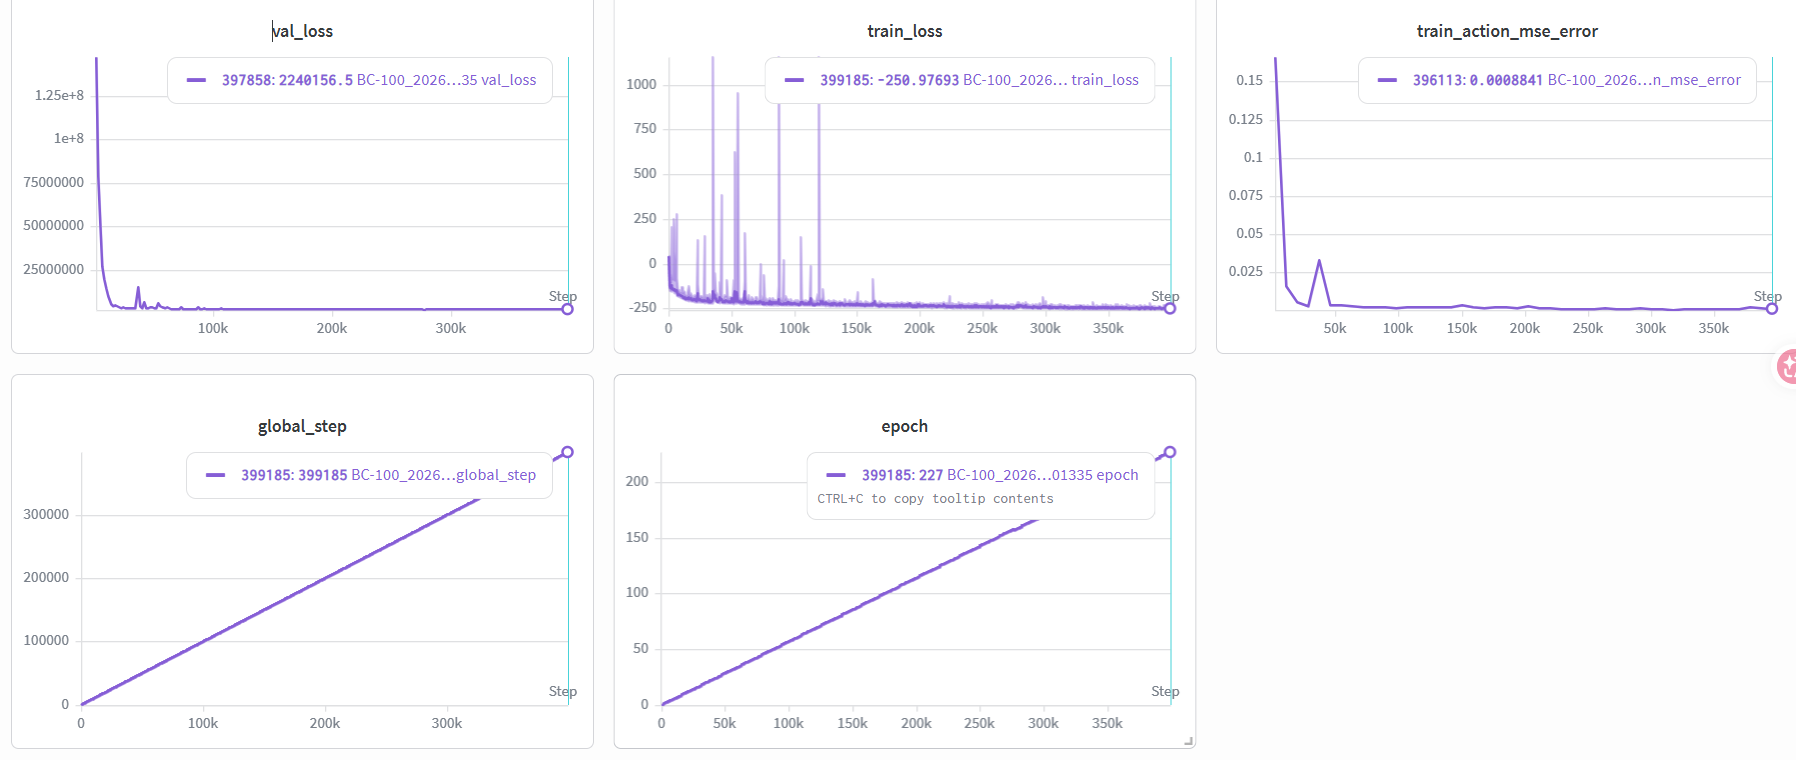
\includegraphics[width=1\linewidth]{bc.png}
    \caption{Training curves of Behavior Cloning, showing low action MSE together with large validation-loss scale and unstable training-loss spikes.}
    \label{fig:bc-train-curves}
\end{figure}

In evaluation, BC did not convert its low local action error into stable long-horizon behavior. This matches the expected weakness of one-step regression: once the hand deviates from the demonstration state distribution, BC keeps predicting the nearest demonstration-like action instead of producing a coherent recovery trajectory. DP should have a better inductive bias for such recovery because it predicts action chunks through denoising, but the current DP checkpoints were still not optimized enough to realize that advantage in successful rollouts.

\subsection{Failure Cases}

The failure cases can be grouped into three levels. The first level contains the better data-coverage DP runs, especially DP-base, DP-mix, and DP-full. These policies usually stayed near the initial pose, hesitated, and made only small progress toward the apple. This is the most informative failure mode because the motion direction was partially aligned with the task, but the policy could not produce a decisive reach-grasp-place trajectory.

The second level contains variants with weaker model capacity, weaker data coverage, or reduced diffusion budget, including DP-depth4, DP-10, and DP-50. These runs more often drifted outward and moved out of the useful \code{cam_high} view. They also produced more joint-limit violations, for example:

\begin{lstlisting}
[2026-05-17 01:21:14,463][mink][DEBUG] - Value -2.36 at joint 27 is outside of its limits: [-2.36, 0.70]
\end{lstlisting}

DP-inf50 and DP-trn50 were between the first two levels. Their training curves were stable, but the rollout behavior did not clearly match DP-base or DP-mix. This is consistent with the trade-off in diffusion steps: reducing training or inference steps can make optimization and sampling cheaper, but it can also reduce the refinement available for precise contact-rich motion.

The third level is BC-100. BC training was computationally heavy and slow, and the rollout behavior showed the least stable hand motion. The hand often moved erratically, and the model produced many values outside joint limits. This supports the conclusion that low one-step action MSE alone is not a sufficient criterion for a dexterous pick-and-place policy.



\section{Option B: Data Efficiency Study}

Option B compares DP-10, DP-50, and DP-full with the same architecture and seed. The only controlled variable is the amount of training data. DP-10 uses 49 episodes, DP-50 uses 246 episodes, and DP-full uses all 491 episodes.

The measured rollout success rate was 0 for all three data-efficiency variants, so the comparison is based on training behavior and observed failure modes rather than successful completions. DP-10 had the weakest data coverage and should be least robust to object-pose and contact-timing variation. DP-50 should recover much of the main approach behavior in simple scenes, while DP-full should be more useful for rare placements and late-stage corrections. The expected data-performance curve is therefore not linear: 50\% of the data should recover a large fraction of the common behavior, but the remaining demonstrations still matter for long-tail robustness.

\appendix

\section{Evaluation Videos}

The submitted videos include one representative rollout for each of the 9 experiments.

\section{Code Listings}

The submitted zip contains only the modified files. The full repository is available at \url{https://github.com/IIvyLEEee/robo_hw2}. The most relevant additions for this report are:

\begin{itemize}[leftmargin=2em]
    \item \code{script/convert_m7_to_zarr.py}: converts the M7 demonstrations into a zarr replay buffer.
    \item \code{diffusion_policy/dataset/m7_star1_dataset.py}: implements the image-state-action dataloader, episode slicing, and validation split.
    \item \code{diffusion_policy/config/image_m7_star1.yaml}: defines the main three-camera Diffusion Policy configuration.
    \item \code{diffusion_policy/config/bc_m7_star1.yaml}: defines the M7 Behavior Cloning baseline.
    \item \code{script/xbot_policy_server.py}: serves trained checkpoints to the XBot evaluation process.
\end{itemize}

\section{Reproducibility Commands}

\subsection{Dataset Preparation}

\begin{lstlisting}
cd /home/liyixuan/robo_hw2/diffusion_policy
conda activate robodiff

python script/convert_m7_to_zarr.py \
  --download-dir data/roboterax_M7_pickplace_example_initial \
  --out-path data/m7_3cam.zarr
\end{lstlisting}

\subsection{Training}

\begin{lstlisting}
# Example: full-data DP baseline
python train.py --config-name=image_m7_star1 \
  exp_name=DP-full \
  training.seed=42 \
  training.device=cuda:0 \
  task.dataset.episode_start=0 \
  task.dataset.episode_end=490 \
  task.dataset.max_train_episodes=null \
  hydra.run.dir=data/outputs/20260516_001335/DP-full \
  logging.name=DP-full_20260516_001335 \
  logging.group=m7_exp \
  logging.mode=online

# Data-efficiency variants
# DP-10: task.dataset.max_train_episodes=49
# DP-50: task.dataset.max_train_episodes=246

# Hyperparameter variants
# DP-trn50:  policy.noise_scheduler.num_train_timesteps=50
# DP-inf50:  policy.num_inference_steps=50
# DP-depth4: policy.n_layer=4

# Behavior Cloning baseline
python train.py --config-name=bc_m7_star1 \
  exp_name=BC-100 \
  training.seed=42 \
  training.device=cuda:0 \
  task.dataset.episode_start=0 \
  task.dataset.episode_end=490 \
  task.dataset.max_train_episodes=null \
  logging.mode=online
\end{lstlisting}

\subsection{Evaluation}

\begin{lstlisting}
# Start policy server from a selected checkpoint.
python script/xbot_policy_server.py \
  -c data/outputs/20260516_001335/DP-full/checkpoints/latest.ckpt \
  -d cuda:0 \
  --bind tcp://*:8003

# Run XBot evaluation.
cd /home/liyixuan/robo_hw2/xbot_sim_benchmark
python scripts/vla_test_xbot.py \
  task=Xbot/XbotPAP \
  vla.server=tcp://127.0.0.1:8003 \
  +app.device=cuda:2 \
  +task.object_select='[1,3]' \
  task.task.params.placement_strategy.params.num_top_objects=1
\end{lstlisting}

\section{AI Assistance Statement}

AI assistance was used for debugging the Isaac Lab and robodiff environments, launching and monitoring the training job, and modifying the codes. The experimental design, final interpretation, and decision to use the marked results remain the author's responsibility.

\end{document}
